% SIAM UQ Supplementary Materials
\documentclass[supplement,review,hidelinks,onefignum,onetabnum]{siamart251216}

\usepackage{amsmath,amssymb}
\usepackage{mathtools}
\usepackage{bm}
\usepackage{graphicx}
\usepackage{booktabs}
\usepackage{enumitem}
\usepackage{algorithm}
\usepackage{algpseudocode}
\usepackage{xr-hyper}
\externaldocument[M-]{part2_analysis}
\externaldocument[I-]{part1_method}


\newcommand{\RR}{\mathbb{R}}
\newcommand{\NN}{\mathbb{N}}
\newcommand{\EE}{\mathbb{E}}
\newcommand{\PP}{\mathbb{P}}
\newcommand{\Var}{\mathrm{Var}}
\newcommand{\Cov}{\mathrm{Cov}}
\newcommand{\tr}{\operatorname{Tr}}
\newcommand{\DKL}{\mathcal{D}_{\mathrm{KL}}}
\newcommand{\diag}{\mathrm{diag}}
\newcommand{\divop}{\operatorname{div}}
\DeclareMathOperator*{\argmin}{arg\,min}
\DeclareMathOperator*{\argmax}{arg\,max}
\newcommand{\gauss}{\gamma}
\renewcommand{\vec}[1]{\bm{#1}}
\newcommand{\mA}{\bm{A}}
\newcommand{\mb}{\bm{b}}
\newcommand{\mh}{\bm{h}}
\newcommand{\mC}{\bm{C}}
\newcommand{\hmC}{\widehat{\bm{C}}}
\newcommand{\mV}{\bm{V}}
\newcommand{\hmV}{\widehat{\bm{V}}}
\newcommand{\mP}{\bm{P}}
\newcommand{\hPperp}{\widehat{\mP}_{\perp}^{\mC}}
\newcommand{\hmP}{\widehat{\bm{P}}}
\newcommand{\mS}{\bm{S}}
\newcommand{\mU}{\bm{U}}
\newcommand{\mR}{\bm{R}}
\newcommand{\mD}{\bm{D}}
\newcommand{\mH}{\bm{H}}
\newcommand{\mL}{\bm{L}}
\newcommand{\mM}{\bm{M}}
\newcommand{\mI}{\bm{I}}
\newcommand{\mW}{\bm{W}}
\newcommand{\mG}{\bm{G}}
\newcommand{\mQ}{\bm{Q}}
\newcommand{\mSigma}{\bm{\Sigma}}
\newcommand{\vzero}{\bm{0}}
\newcommand{\cond}{\operatorname{cond}}
\newcommand{\vx}{\bm{x}}
\newcommand{\vy}{\bm{y}}
\newcommand{\vn}{\bm{n}}
\newcommand{\vz}{\bm{z}}
\newcommand{\vZ}{\bm{Z}}
\newcommand{\vu}{\bm{u}}
\newcommand{\vU}{\bm{U}}
\newcommand{\vY}{\bm{Y}}
\newcommand{\vv}{\bm{v}}
\newcommand{\vw}{\bm{w}}
\newcommand{\vtheta}{\bm{\theta}}
\newcommand{\whvtheta}{\widehat{\bm{\theta}}}
\newcommand{\scL}{\mathcal{L}}
\newcommand{\scZ}{\mathcal{Z}}
\newcommand{\scS}{\mathcal{S}}
\newcommand{\scF}{\mathcal{F}}
\newcommand{\St}{\mathrm{St}}
\newcommand{\Gr}{\mathrm{Gr}}

% Additional macros used in moved appendices (App E, F, G)
\newcommand{\hbeta}{\widehat{\beta}}
\newcommand{\vW}{\bm{W}}
\newcommand{\veta}{\bm{\eta}}
\newcommand{\vb}{\bm{b}}
\newcommand{\ve}{\bm{e}}
\DeclareMathOperator{\range}{range}
\newcommand{\hmA}{\widehat{\bm{A}}}
\newcommand{\hmM}{\widehat{\bm{M}}}
\newcommand{\hmb}{\widehat{\bm{b}}}
\newcommand{\mB}{\bm{B}}
\newcommand{\hvbeta}{\widehat{\bm{\theta}}^{r}}

\setlength{\emergencystretch}{3em}
\newcommand{\creflastconjunction}{, and~}

\newsiamremark{remark}{Remark}
\newsiamremark{assumption}{Assumption}
\crefname{remark}{Remark}{Remarks}
\crefname{assumption}{Assumption}{Assumptions}
% Cleveref types labels in \newsiamremark environments by the shared theorem
% counter, so \Cref of a remark or assumption prints "Theorem N". Alias the
% counter to the correct type inside each environment (the alias is local to
% the environment group), which makes \Cref print Remark/Assumption.
\let\origremarkenv\remark
\renewcommand{\remark}{\crefalias{theorem}{remark}\origremarkenv}
\let\origassumptionenv\assumption
\renewcommand{\assumption}{\crefalias{theorem}{assumption}\origassumptionenv}

\headers{Copula Active Subspaces}{J.~Chen and P.~J.~van Leeuwen}
\title{Copula Active Subspaces II: Error Decomposition, A Posteriori Estimation, and Sharpness of the Bounds\thanks{Submitted to the editors \today. \funding{This work was supported by the Consortium for Advanced Data Assimilation Research and Education (CADRE), funded by NOAA under grant 2007893.}}}
\author{%
  Joshua Chen\thanks{Department of Atmospheric Science, Colorado State University, Fort Collins, CO 80523 (\email{Joshua.Chen@colostate.edu}).}
  \and
  Peter Jan van Leeuwen\thanks{Department of Atmospheric Science, Colorado State University, Fort Collins, CO 80523 (\email{Peter.vanLeeuwen@colostate.edu}).}
}

\begin{document}
\maketitle

\Cref{sm:rate-real} checks the $N^{-1/2}$ subspace-recovery rate of \Cref{M-lem:score-cov-rate} on a law whose copula score lies in $\scF_\Lambda$. \Cref{sm:disintegration-mc} describes the computation of the reference values, and \Cref{sm:sharper-bound} compares the sharper bound of \cite{LiCuiLiMarzoukZahm2024sharp} with the trace bound minimized by the estimator, giving the numbers of \S\ref{M-sec:tightness} of the main manuscript. \Cref{sm:experimental-protocol} gives the seeds, tuning parameters and hardware, and \Cref{sm:composite-anatomy} reports the decomposition on Examples~2 and~3.
Throughout, $\vn$ denotes the observation noise in its original coordinates, before the rank transform, with law $\pi_{\vn}$, and all other notation follows the main manuscript. Numbers with the SM prefix (\S\ref{sm:rate-real}, \Cref{tab:sm-jhi}, \eqref{eq:sm-logcZ}) refer to these supplementary materials, and numbers without it refer to the main manuscript.

% =====================================================================
\section{Numerical check of the Stage-1 rate}
\label{sm:rate-real}

We check the Stage-1 statistical rate on a law whose copula score lies in $\scF_\Lambda$, so that the measured error contains no truncation error. \Cref{fig:pedagogical} illustrates the estimator in two dimensions. Results on the three example problems, including subspace recovery and the convergence of the parameterized eigenspace in $(K_1,q_1)$, are in Part~I \cite{CAS_partI} and its supplement; \Cref{sm:experimental-protocol} specifies the reference bases of the example problems.

\begin{figure}[h]
\centering
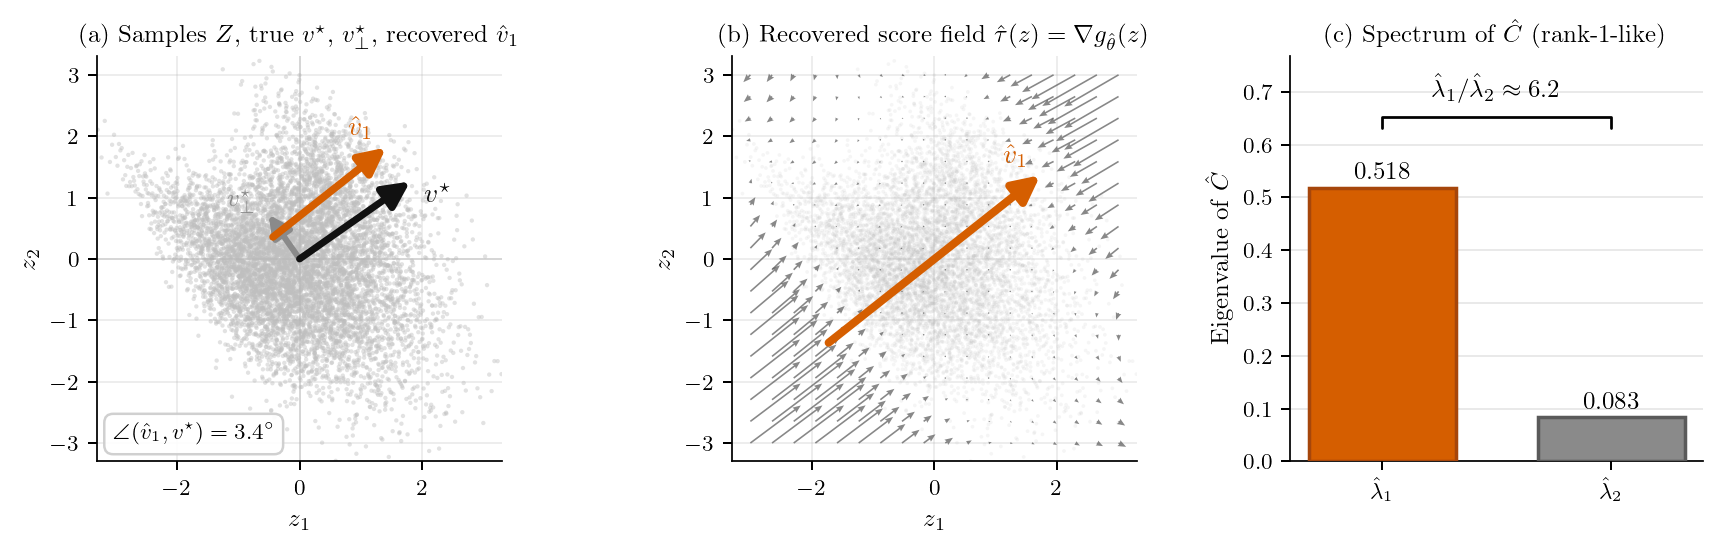
\includegraphics[width=\textwidth]{pedagogical_2d.png}
\caption{\textsc{Cas} in two dimensions on a rank-$1$ non-Gaussian copula with quadratic conditional-mean dependence in a non-axis-aligned direction $\vv^\star$: (a)~samples and the top eigenvector $\widehat{\vv}_1$ of $\hmC$, (b)~estimated score field, (c)~spectrum of $\hmC$.}
\label{fig:pedagogical}
\end{figure}

\Cref{M-lem:score-cov-rate} of the main paper gives an $O_p(N^{-1/2})$ rate for $\|\sin\Theta(\hmV_r^{\mC}, \mV_{r,\Lambda})\|_F$ at a fixed Hermite multi-index set $\Lambda$. We check this rate on a Gaussian-copula law, for which the truncation error is exactly zero. \begin{remark}[Gaussian-copula reduction]
\label{rem:gaussian-copula}
If $\pi_{\vZ} = \gauss(0,\bm\Sigma^{\vZ})$ for a correlation matrix $\bm\Sigma^{\vZ} := \EE_{\pi_{\vZ}}[\vZ\otimes\vZ]$, the log-copula with respect to $\gauss_d$ is the quadratic $g^\star(\vz) = -\tfrac12\vz^\top \mM\vz + \mathrm{const}$ with $\mM := (\bm\Sigma^{\vZ})^{-1} - \mI$, a combination of degree-$2$ Hermite polynomials, since $z_iz_j = H_{e_i+e_j}$ ($i\ne j$) and $z_i^2 = \sqrt2 H_{2e_i} + 1$. The span $\{\nabla H_\alpha : |\alpha|=2\}\subset\scF_\Lambda$ for any $\Lambda = \Lambda_{K,q}$ with $K, q \ge 2$ contains every symmetric linear vector field $\vz \mapsto \bm S\vz$, $\bm S = \bm S^\top$ (the gradients of quadratics), so $\scS(\vz) = -\mM\vz \in \scF_\Lambda$, since $\mM$ is symmetric. Hence $\scS_\Lambda = \scS$, with $\theta^\star$ supported on degree $2$, and $\mC = \mM\,\bm\Sigma^{\vZ}\mM$. By Fisher consistency \cite[Thm.~2, Cor.~3]{Hyvarinen2005}, the unique infinite-sample minimizer of the strictly convex quadratic objective equals $\theta^\star$; by the closed form of the solve and the strong law of large numbers, $\widehat\theta \to \theta^\star$ a.s.\ and $\hmC \to \mC$ in operator norm as $\tau_N \to 0$; at the fixed strength $\tau_N \asymp \kappa\|\hmA\|_{\rm op}$ used here, the bias term of \Cref{M-lem:score-cov-rate} is $O(\tau_N)$ and does not vanish, but it does not visibly change the measured rate of \Cref{fig:rate-sm} over the sample sizes used.
\end{remark}
Then $\mV_{r,\Lambda} = \mV_r^{\mC}$, the top-$r$ eigenspace of the closed-form $\mC$, computed without Monte Carlo, and the recovery error is purely statistical. On a single correlated block of $3$ coordinates ($d = 20$, $r = 3$, within-block off-diagonal $\rho = 0.7$, the remaining $17$ coordinates independent) we vary $N$ over a geometric grid with $(K_1, q_1) = (2, 2)$ and $20$ repetitions for each $N$, and compute $\|\sin\Theta(\hmV_r^{\mC}, \mV_r^{\mC})\|_F$ relative to this analytic reference. The least-squares line in log-log coordinates has slope $-0.502$ (\Cref{fig:rate-sm}), which agrees with the rate $-1/2$ of \Cref{M-lem:score-cov-rate}.

\begin{figure}[h]
\centering
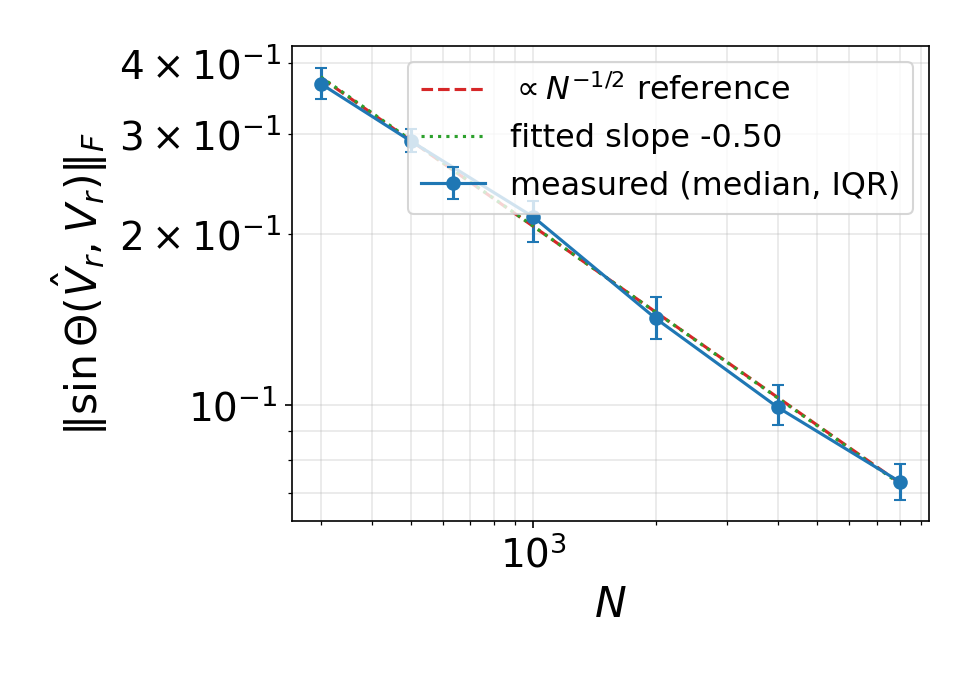
\includegraphics[width=\textwidth]{rate_plot.png}
\caption{Empirical verification of the $O_p(N^{-1/2})$ subspace-recovery rate of \Cref{M-lem:score-cov-rate} on a Gaussian-copula law ($d = 20$, $r = 3$: one block of $3$ coordinates with within-block $\rho = 0.7$, the remaining $17$ independent), where the copula score is linear so $\mV_{r,\Lambda} = \mV_r^{\mC}$ exactly and the exact $\mV_r^{\mC}$ is the closed-form top-$r$ eigenspace of $\mC = \mM\,\bm\Sigma^{\vZ}\mM$, $\mM = (\bm\Sigma^{\vZ})^{-1}-\mI$ (\Cref{rem:gaussian-copula}). Measured $\|\sin\Theta(\hmV_r^{\mC}, \mV_r^{\mC})\|_F$ (median, IQR over $20$ repetitions) with a reference line $\propto N^{-1/2}$ and the least-squares slope in log-log coordinates.}
\label{fig:rate-sm}
\end{figure}

% =====================================================================
\section{Reference divergences in rank-Gaussianized coordinates}
\label{sm:disintegration-mc}

The reference values of \S\ref{M-sec:tightness} and \S\ref{M-sec:exp-composite} of the main manuscript and of \Cref{sm:sharper-bound,sm:composite-anatomy} are the Stage-1 divergence $\DKL(\pi_{\vn}\,\|\,\pi_{\vn}(\,\cdot\,;\mV_r))$ and the reduced-density divergence $\mathcal E_{\rm dens}$, computed on the known noise law. Both require $\pi_{\vU}(\vu) := \int \pi_{\vZ}(\mV_r\vu + \mV_\perp\vw)\,\mathrm{d}\vw$, the marginal of the rank-Gaussianized $\pi_{\vZ}$ along $\mV_r$, at given points.

The rank transform is applied before that integral is evaluated. Writing $f_k$ and $F_k$ for the exact marginal density and distribution function of the mixed latent coordinate $z_k$, built as a Gaussian mixture over the active block, the transform is $Z_k = \Phi^{-1}(F_k(z_k))$ on the $b = 8$ mixed coordinates and the identity on the $12$ unmixed coordinates, whose marginals are already standard Gaussian. Those $12$ coordinates are independent of the mixed block, so the copula density depends on the mixed block alone, and
\begin{equation}
  \log c^{Z}(\vZ) \;=\; \log\pi_{\vz}(\vz) \;-\; \textstyle\sum_{k<b}\log f_k(z_k),
  \qquad z_k = F_k^{-1}(\Phi(Z_k)),
  \label{eq:sm-logcZ}
\end{equation}
since the standard-Gaussian factors of the two changes of variables cancel.

The integral over the complement is a Gaussian expectation of the copula density. Under the orthogonal splitting $\gauss_b = \gauss_r\otimes\gauss_{b-r}$, with $\mathbf A$ the mixed-block rows of $\mV_r$,
\begin{equation}
  c_r^{U}(\vu) \;=\; \EE_{\bm\xi \sim \gauss(\vzero,\, \mI_b - \mathbf A\mathbf A^\top)}\bigl[\,c^{Z}(\mathbf A\vu + \bm\xi)\,\bigr],
  \qquad
  \log\pi_{\vU}(\vu) = \log c_r^{U}(\vu) + \log\gauss_r(\vu),
  \label{eq:sm-crU}
\end{equation}
evaluated by a tensor Gauss--Hermite rule \cite{GolubWelsch1969} in the eigenbasis of $\mI_b - \mathbf A\mathbf A^\top$. At $\mV_r^{\mC}$ that matrix has $b-r$ unit eigenvalues and $r$ zeros, so the rule runs over $b - r = 4$ axes, with eleven nodes on each. For an estimated basis, the $r$ zero eigenvalues become positive, equal to the squared singular values of the rows of the basis on the $12$ unmixed coordinates, and are largest at small $N$. The rule then uses seven nodes on each of the $b-r$ leading axes, three on any other axis with nonzero variance, and one on the remaining axes.

The Stage-1 divergence follows as the outer average of the conditional divergence,
\begin{equation}
  \DKL\bigl(\pi_{\vn}\,\|\,\pi_{\vn}(\,\cdot\,;\mV_r)\bigr)
  \;=\;
  \EE_{\pi_{\vU}}\Bigl[\,\EE_{\bm\xi}\bigl[\rho\log\rho\bigr]\,\Bigr],
  \qquad \rho := c^{Z}(\mathbf A\vu+\bm\xi)/c_r^{U}(\vu),
  \label{eq:sm-delta-sub}
\end{equation}
over $\vu = \mV_r^\top\vZ$ with $\vZ$ drawn from $\pi_{\vZ}$.
The inner expectation of \eqref{eq:sm-delta-sub} uses the nodes and weights of \eqref{eq:sm-crU}, so it requires no further evaluations of the density. It is also nonnegative at every $\vu$, whereas the difference $\log c^{Z} - \log c_r^{U}$, which could be averaged instead, can take either sign. We computed both forms in the same run, with outer sample size $4000$ and seed $20260806$. Their means differ by less than twice the standard error of the signed form on each example, and the standard error of the conditional form is smaller by factors between $9$ and $19$. The reduced-density divergence $\mathcal E_{\rm dens}$ is the outer average of $\log\pi_{\vU}(\vu_m) - \log\widehat\pi_{\vU}(\vu_m)$ on the same points, with $\widehat\pi_{\vU}$ from the Stage-2 closed form \eqref{I-eq:stage2-closedform} of Part~I.

The divergences are computed after the rank transform. The marginals of the latent coordinates $\vz = \mQ\vW$ are logistic on the $12$ unmixed coordinates, and the rotation changes them on the mixed block. In the latent coordinates the complement of the active subspace is standard Gaussian and independent of it, so the reduction loses nothing there; after the rank transform it does. At $\mV_r^{\mC}$ the two computations therefore differ by the whole divergence.

% =====================================================================
\section{A sharper a posteriori KL divergence bound}
\label{sm:sharper-bound}

The main paper uses the Gaussian-reference KL divergence bound
\begin{equation}
  \DKL\bigl(\pi_{\vZ}\,\|\,\pi_{\vZ}(\,\cdot\,;\mV_r)\bigr) \;\le\; \tfrac12\tr((\mI-\mV_r\mV_r^\top)\mC),
  \label{eq:sm-trace-bound}
\end{equation}
with $\pi_{\vZ}(\vz;\mV_r) := c_r^{U}(\mV_r^\top\vz)\,\gauss_d(\vz)$ the reduced model \eqref{I-eq:pi-star-form} in $\vZ$-coordinates. This bound is used in the rate analysis (\Cref{sm:rate-real}), and it gives the basis in closed form, as the top-$r$ eigenvectors of $\hmC$. When $\pi_{\vZ}$ has finite second moment and finite Fisher information in the directions orthogonal to the span of $\mV_r$, the dimensional log-Sobolev refinement of \cite{LiCuiLiMarzoukZahm2024sharp} gives a tighter upper bound, computable on the examples. Writing
\[
  \Sigma^{Z}_{\perp} := \mV_\perp^\top \EE_{\pi_{\vZ}}[\vZ\otimes \vZ]\mV_\perp,
  \qquad
  F^{Z}_{\perp} := \mV_\perp^\top \EE_{\pi_{\vZ}}[s(\vZ)\otimes s(\vZ)]\mV_\perp,
  \qquad s := \nabla \log \pi_{\vZ},
\]
for any $\mV_r$ with orthogonal complement $\mV_\perp$, \cite{LiCuiLiMarzoukZahm2024sharp} gives two functionals
\begin{align}
  J_{\mathrm{lo}}(\mV_r)
  &= \tfrac12\bigl[\,\tr(\Sigma^Z_\perp - \mI_{d-r}) - \log\det \Sigma^Z_\perp\,\bigr], \nonumber \\
  J_{\mathrm{hi}}(\mV_r)
  &= \tfrac12\bigl[\,\tr(\Sigma^Z_\perp - \mI_{d-r}) + \log\det F^Z_\perp\,\bigr],
  \label{eq:sm-jhi-jlo}
\end{align}
that satisfy, for every $\mV_r$,
\begin{equation}
  J_{\mathrm{lo}}(\mV_r)
  \;\le\;
  \DKL\!\bigl(\pi_{\vZ}\,\|\,\pi^\star_{Z, \mV_r}\bigr)
  \;\le\;
  J_{\mathrm{hi}}(\mV_r)
  \;\le\;
  \tfrac12\tr((\mI-\mV_r\mV_r^\top)\mC).
  \label{eq:sm-jhi-sandwich}
\end{equation}
The rightmost inequality follows from an algebraic identity. With $\psi(\lambda) := \lambda - 1 - \log\lambda \ge 0$,
\begin{equation}
  \tfrac12\tr((\mI-\mV_r\mV_r^\top)\mC) - J_{\mathrm{hi}}(\mV_r)
  \;=\;
  \tfrac12 \sum_{i=1}^{d-r}\psi(\lambda_i(F^Z_\perp)),
  \label{eq:sm-jhi-trace-gap}
\end{equation}
so the gap is zero exactly when $F^Z_\perp = \mI_{d-r}$ (the remaining Fisher information matches the Gaussian reference) and grows monotonically with the eigenvalue spread of $F^Z_\perp$. For a centered non-singular Gaussian $\pi_{\vZ}$, the upper bound is exact at every $\mV_r$, $J_{\mathrm{hi}}(\mV_r) = \DKL(\pi_{\vZ}\,\|\,\pi^\star_{Z,\mV_r})$ \cite{LiCuiLiMarzoukZahm2024sharp}.

The functional $J_{\mathrm{hi}}$ has no closed-form minimizer in $\mV_r$, unlike the trace bound \eqref{eq:sm-trace-bound}. Its value at a given $\mV_r$ requires the moments $\Sigma^Z_\perp$ and $F^Z_\perp$, and its minimization requires iteration. We take both moments at the rank-Gaussianized $\vZ$ with the exact copula score of \Cref{sm:disintegration-mc}, so the values below contain no score-estimation error.

\paragraph{Bounds for $\mV_r^{\mC}$ and for the minimizer of $J_{\mathrm{hi}}$} On each of the three examples we evaluate $J_{\mathrm{hi}}$ and the trace bound at the top-$r$ eigenvectors $\mV_r^{\mC}$ of $\mC$, which minimize the trace bound in closed form, and at the minimizer $\mV_{r,\rm hi}$ of $J_{\mathrm{hi}}$, obtained by Riemannian gradient descent \cite{AbsilMahonySepulchre2008} started at $\mV_r^{\mC}$. \Cref{tab:sm-jhi} reports both, together with the reference divergence of \Cref{sm:disintegration-mc}. The descent terminates when the Riemannian gradient norm falls below $10^{-10}$.

\begin{table}[h]
\centering\small
\caption{The trace bound, $J_{\mathrm{hi}}$ and the reference divergence at $\mV_r^{\mC}$ on Examples~1--3. The gap column is $\tfrac12\sum_i\psi(\lambda_i(F^Z_\perp))$ of \eqref{eq:sm-jhi-trace-gap}, computed from the eigenvalues of $F^Z_\perp$, which avoids cancellation. Sampling noise spreads the estimated eigenvalues and so tends to increase this sum. The last column is the principal-angle distance from $\mV_r^{\mC}$ to the minimizer of $J_{\mathrm{hi}}$, at which $J_{\mathrm{hi}}$ agrees with its value at $\mV_r^{\mC}$ to four decimal places. Divergences and bounds in nats.}
\label{tab:sm-jhi}
\begin{tabular}{l|ccc|c|c}
\toprule
Example & trace bound & $J_{\mathrm{hi}}$ & gap & $\DKL$ at $\mV_r^{\mC}$ & $\|\sin\Theta\|_F$ \\
\midrule
Example~1 & $0.0181$ & $0.0181$ & $4.9\cdot10^{-5}$ & $0.0095{\pm}0.0001$ & $0.011$ \\
Example~2 & $0.0451$ & $0.0449$ & $2.0\cdot10^{-4}$ & $0.0275{\pm}0.0004$ & $0.011$ \\
Example~3 & $0.0182$ & $0.0181$ & $7.3\cdot10^{-5}$ & $0.0092{\pm}0.0002$ & $0.009$ \\
\bottomrule
\end{tabular}
\end{table}

\paragraph{Comparison}

The gap \eqref{eq:sm-jhi-trace-gap} is below $0.5\%$ of the trace bound on each example, and every eigenvalue of $F^Z_\perp$ lies in $[0.995, 1.024]$. Twelve of the sixteen complement directions are unmixed coordinates with scores $-W_j$, so their eigenvalues equal $1$, and the other four differ from $1$ by at most $0.024$. When the conditional laws in the complement directions are further from standard Gaussian, $\|F^Z_\perp - \mI\|_F$ is larger and, by \eqref{eq:sm-jhi-trace-gap}, so is the gap.

The trace bound exceeds the divergence by factors of $1.91$, $1.64$ and $1.98$, and $J_{\mathrm{hi}}$ by $1.90$, $1.63$ and $1.97$. The excess comes from the Gaussian logarithmic Sobolev inequality behind \eqref{eq:sm-trace-bound}, and the sharper bound does not remove it.

The minimizer of $J_{\mathrm{hi}}$ lies within $\|\sin\Theta\|_F \le 0.011$ of $\mV_r^{\mC}$ on all three examples, and the values of $J_{\mathrm{hi}}$ at the two bases agree to four decimal places, so the closed-form basis of the estimator also minimizes the sharper functional to that accuracy.

\section{Experimental Protocol}
\label{sm:experimental-protocol}

All experiments are deterministic under fixed random seeds, listed below. Rank-Gaussianization uses average ranks for ties and the $k/(N+1)$ plotting-position convention. The randomized range finder \cite{HalkoMartinssonTropp2011} uses oversampling $p = 10$ and $q_{\text{pwr}} = 2$ power-iteration steps. Implementation is in Python (NumPy/SciPy 1.13), and the code is available at the repository given in the Reproducibility section of the main manuscript.

\paragraph{Example problems and reference bases (\Cref{sm:rate-real})} The setup uses $d = 20$ with the Example~1 block of Part~I \cite{CAS_partI} (two inputs at coordinates $(0, 1)$, two outputs at $(2, 3)$), curvature $a = 0.7$, saturation scale $M = 2.5$, a uniformly random rotation $\mQ \sim \mathrm{Unif}(\mathrm{O}(8))$ mixing the first $b=8$ coordinates (identity on the remaining $12$), and logistic marginals. The active rank is $r^\star = 4$. Because $\mQ$ is orthogonal, $\EE[\vZ\vZ^\top] = \mI_{20}$ and the active subspace is not aligned with the coordinate axes but can be recovered exactly. The exact basis $\mV_r^{\mC}$ is the top-$r$ eigenspace of $\mC$, computed once from $N_{\rm ref} = 10^6$ samples of the closed-form score, and the quantities of \S\ref{M-sec:tightness} of the main manuscript and of \Cref{sm:sharper-bound} are computed for it. The Stage-2 reference values are computed for the top-$r$ eigenbasis $\mV_{r,\Lambda}$ of $\mC_\Lambda$ for $(K_1, q_1) = (4,2)$, estimated by Hermite score matching from $N_{\rm ref} = 10^6$ samples.

\paragraph{Sharper-bound evaluation (\Cref{sm:sharper-bound})} The moments behind \Cref{tab:sm-jhi} are computed at the rank-Gaussianized $\vZ$ of \Cref{sm:disintegration-mc}, with $2\cdot10^6$ samples and seed $0$. They cannot be computed in the latent coordinates $\vz = \mQ\vW$ instead, even though the scores have closed forms there. Under an orthogonal $\mQ$ the copula score in $\vz$ is $\mQ$ applied to the score in the latent coordinates, whose components on the $12$ unmixed coordinates cancel identically. The matrix $\mC$ would then have rank $r^\star$, and the trace bound at its leading eigenspace would be zero to machine precision. After the exact rank transform this does not happen, because the marginals on the mixed block are not Gaussian.

The two bounds share the term $\tr(\Sigma^Z_\perp - \mI)$, a difference of two traces of order $d-r$ whose value is of order $10^{-2}$, so forming each bound separately loses three significant figures to cancellation. Their difference \eqref{eq:sm-jhi-trace-gap} contains no such cancellation, every summand $\psi(\lambda_i)$ being nonnegative, and is evaluated that way. The trace bound itself is formed as $\tfrac12\tr((\mI-\mV_r\mV_r^\top)\mC)$, a sum of nonnegative terms.

\paragraph{A priori terms (\S\ref{M-sec:exp-aposteriori} of the main manuscript)} The Hermite truncation term of \eqref{M-eq:stage1-threeterm} is computed from $N_{\rm ref} = 10^6$ samples of the closed-form score. Its square is the difference between $\tr(\mC_\Lambda)$ for the largest multi-index set $\Lambda_{6,3}$ and for the selected set $\Lambda_{4,2}$.

\paragraph{Stage-2 normalizer (\S\ref{M-sec:aposteriori} of the main manuscript)} The normalizer $\widehat Z_r = \EE_{\gauss_r}[\exp(\widehat\scL_r)]$ is computed by a scrambled Sobol' sequence \cite{Sobol1967, Owen1995} with $M_{\rm norm} = 8192$ points: the points of $[0,1]^r$ are mapped componentwise through $\Phi^{-1}$, the scramble is seeded by the model seed, and the constraints of the Stage-2 solve, $\scL_r \le \tau$ on a ball and the margin on the leading form, bound the integrand above (Part~I \cite{CAS_partI}). The normalizer is used only to evaluate $\log\widehat\pi_{\vU}$ and $\log\widehat\pi_{\vn}$; no estimation step uses it.

\paragraph{Computation} The Stage-1 and Stage-2 estimates are computed in one pass over the sample, in batches. The decompositions of the different estimated models, and the rate check, run in parallel. The computation over the sequence of larger multi-index sets estimates the peak memory for each set before starting it and skips any set that would exceed $35$~GB. No set reported here was skipped, the largest being $\Lambda_{6,3}$ with $25{,}770$ multi-indices.

% =====================================================================
\section{The three terms on Examples 2 and 3}
\label{sm:composite-anatomy}
\Cref{fig:composite-ex2,fig:composite-ex3} report Examples~2 and~3 under the protocol of \Cref{M-fig:composite-main} of the main manuscript. The reference values of $\mathcal E_{\rm marg}$, $\mathcal E_{\rm proj}$, $\mathcal E_{\rm dens}$ and of the total divergence are computed as in \Cref{sm:disintegration-mc} on one evaluation sample, and $\mathcal E_{\rm tot} := \mathcal E_{\rm marg} + \mathcal E_{\rm proj} + \mathcal E_{\rm dens}$. The reference value of $\mathcal E_{\rm marg}$ omits $R_N$ and $\log A$ (\Cref{M-prop:exact-decomp}). The term $\mathcal E_{\rm dens}$ is evaluated at the basis $\mV_{r,\Lambda}$ of \S\ref{M-sec:exp-reference} of the main manuscript, and its change between $\mV_{r,\Lambda}$ and $\hmV_r^{\mC}$ is the basis perturbation $\Delta_{\rm cpl}$. The difference between $\mathcal E_{\rm tot}$ and the reference total contains $R_N$, $\log A$ and $\Delta_{\rm cpl}$.

\begin{figure}[h]
\centering
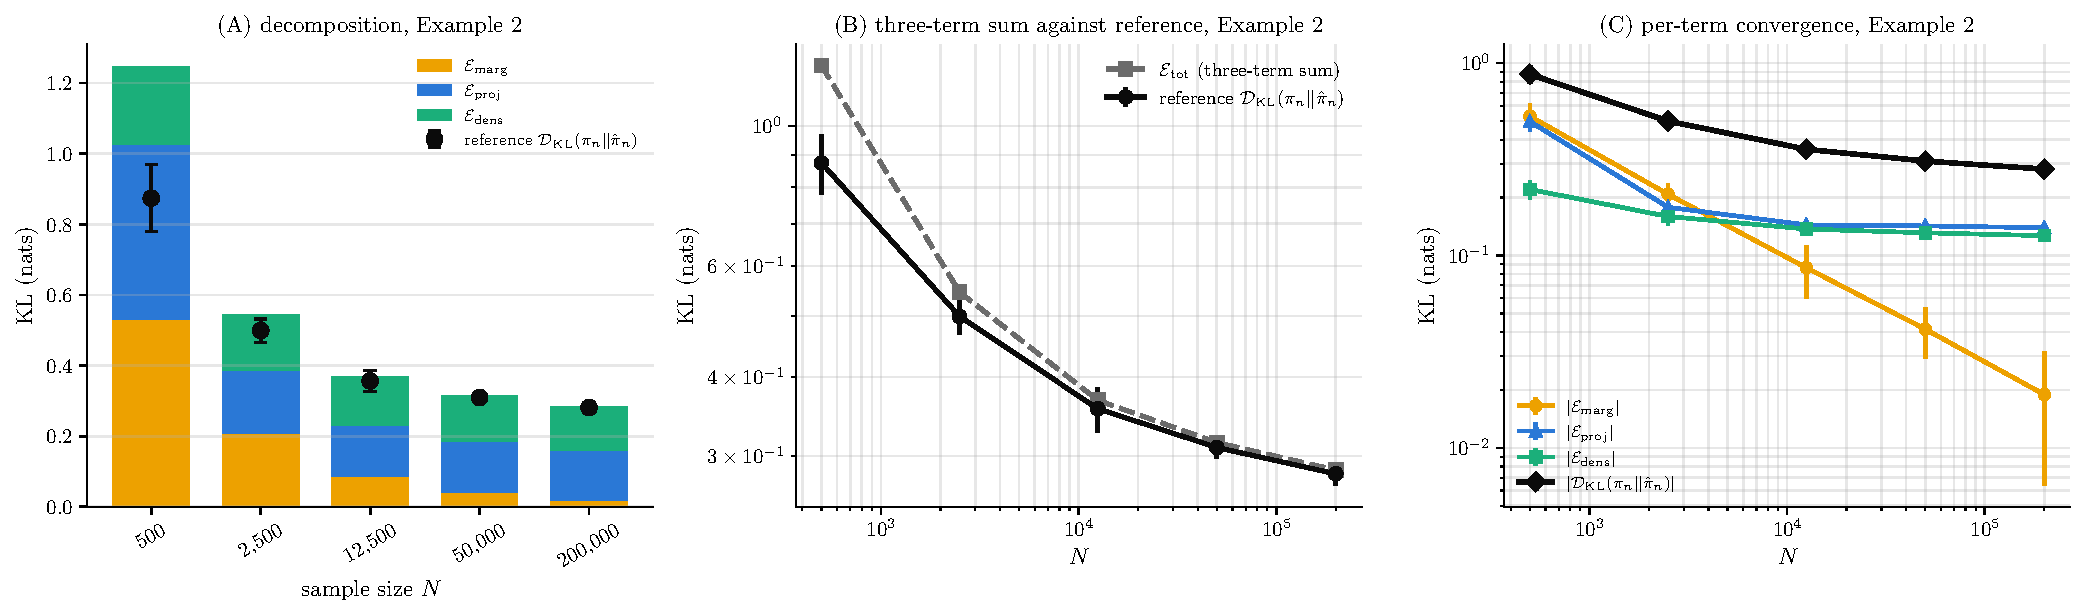
\includegraphics[width=\textwidth]{figSy_v2_even_fold.pdf}
\caption{Reference values of the three terms of the KL divergence decomposition on Example~2. The marginal term $\mathcal E_{\rm marg}$ is the largest term for $N \le 2500$ and decreases toward zero as $N$ grows. The subspace term $\mathcal E_{\rm proj}$ approaches a limit set by the trailing eigenvalues of $\mC_\Lambda$ and is the largest term from $N \geq 12{,}500$, and $\mathcal E_{\rm dens}$ approaches a limit slightly below it. For $N \ge 12{,}500$ the three-term sum $\mathcal E_{\rm tot}$ and the reference total $\DKL$ nearly coincide.}
\label{fig:composite-ex2}
\end{figure}

\begin{figure}[h]
\centering
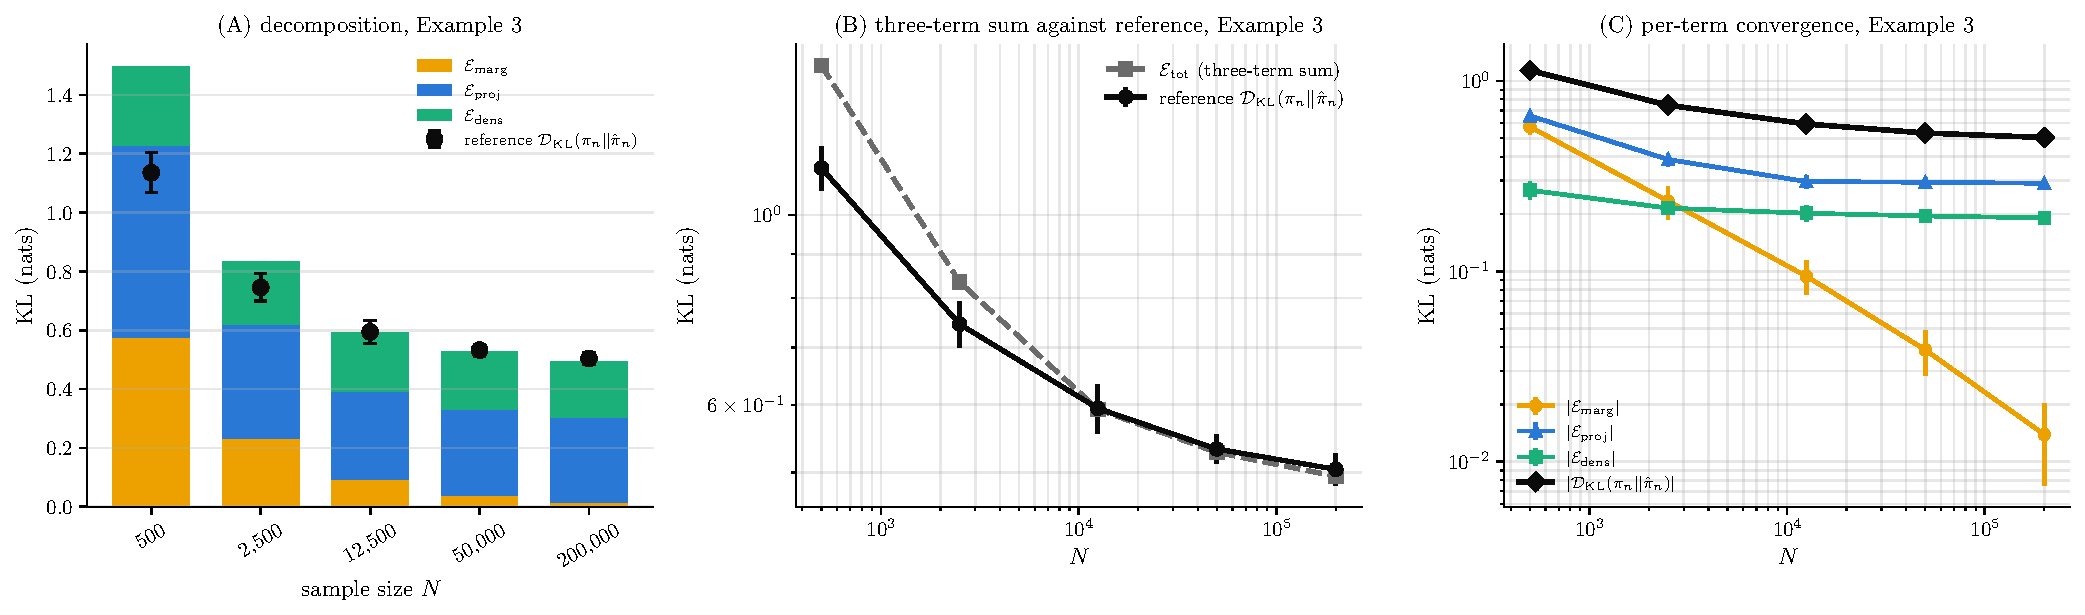
\includegraphics[width=\textwidth]{figSy_v2_conformal_cube.pdf}
\caption{Reference values of the three terms of the KL divergence decomposition on Example~3. The subspace term $\mathcal E_{\rm proj}$ is the largest term at every $N$ and approaches a limit set by the trailing eigenvalues of $\mC_\Lambda$. The marginal term $\mathcal E_{\rm marg}$ decreases toward zero and falls below $\mathcal E_{\rm dens}$ between $N = 2500$ and $N = 12{,}500$. As on Example~2, $\mathcal E_{\rm tot}$ and $\DKL$ nearly coincide for $N \ge 12{,}500$.}
\label{fig:composite-ex3}
\end{figure}


\begin{thebibliography}{10}

\bibitem{AbsilMahonySepulchre2008}
{\sc P.-A. Absil, R.~Mahony, and R.~Sepulchre}, {\em Optimization Algorithms on Matrix Manifolds}, Princeton University Press, Princeton, NJ, 2008.

\bibitem{CAS_partI}
{\sc J.~Chen and P.~J. van Leeuwen}, {\em Copula Active Subspaces I: A score-covariance method for reduced-order non-{G}aussian density estimation}, submitted to SIAM/ASA J. Uncertain. Quantif.; preprint, arXiv:2609.36142, 2026.

\bibitem{GolubWelsch1969}
{\sc G.~H. Golub and J.~H. Welsch}, {\em Calculation of {G}auss quadrature rules}, Math. Comp., 23 (1969), pp.~221--230.

\bibitem{HalkoMartinssonTropp2011}
{\sc N.~Halko, P.-G. Martinsson, and J.~A. Tropp}, {\em Finding structure with randomness: Probabilistic algorithms for constructing approximate matrix decompositions}, SIAM Rev., 53 (2011), pp.~217--288.

\bibitem{Hyvarinen2005}
{\sc A.~Hyv\"arinen}, {\em Estimation of non-normalized statistical models by score matching}, J. Mach. Learn. Res., 6 (2005), pp.~695--709.

\bibitem{LiCuiLiMarzoukZahm2024sharp}
{\sc M.~T.~C. Li, T.~Cui, F.~Li, Y.~Marzouk, and O.~Zahm}, {\em Sharp detection of low-dimensional structure in probability measures via dimensional logarithmic {S}obolev inequalities}, Inf. Inference, 14 (2025), iaaf021.

\bibitem{Owen1995}
{\sc A.~B. Owen}, {\em Randomly permuted $(t,m,s)$-nets and $(t,s)$-sequences}, in Monte Carlo and Quasi-Monte Carlo Methods in Scientific Computing, H.~Niederreiter and P.~J.-S. Shiue, eds., Lecture Notes in Statist. 106, Springer, New York, 1995, pp.~299--317.

\bibitem{Sobol1967}
{\sc I.~M. Sobol'}, {\em On the distribution of points in a cube and the approximate evaluation of integrals}, USSR Comput. Math. Math. Phys., 7 (1967), pp.~86--112.

\end{thebibliography}


\end{document}
